\documentclass[11pt,letterpaper]{article}
\usepackage[lmargin=1in,rmargin=1in,tmargin=1in,bmargin=1in]{geometry}
\usepackage{../style/homework}
\usepackage{../style/commands}
\setbool{quotetype}{true} % True: Side; False: Under
\setbool{hideans}{false} % Student: True; Instructor: False

% -------------------
% Content
% -------------------
\begin{document}

\homework{10: Due 06/14}{Somewhere, something incredible is waiting to be known.}{Carl Sagan}

% Problem 1
\problem{10} Sketch the function $f(x)= \dfrac{11}{3} \left( \dfrac{1}{2} \right)^x$ as accurately as possible on the graph below. 
	\[
	\fbox{
	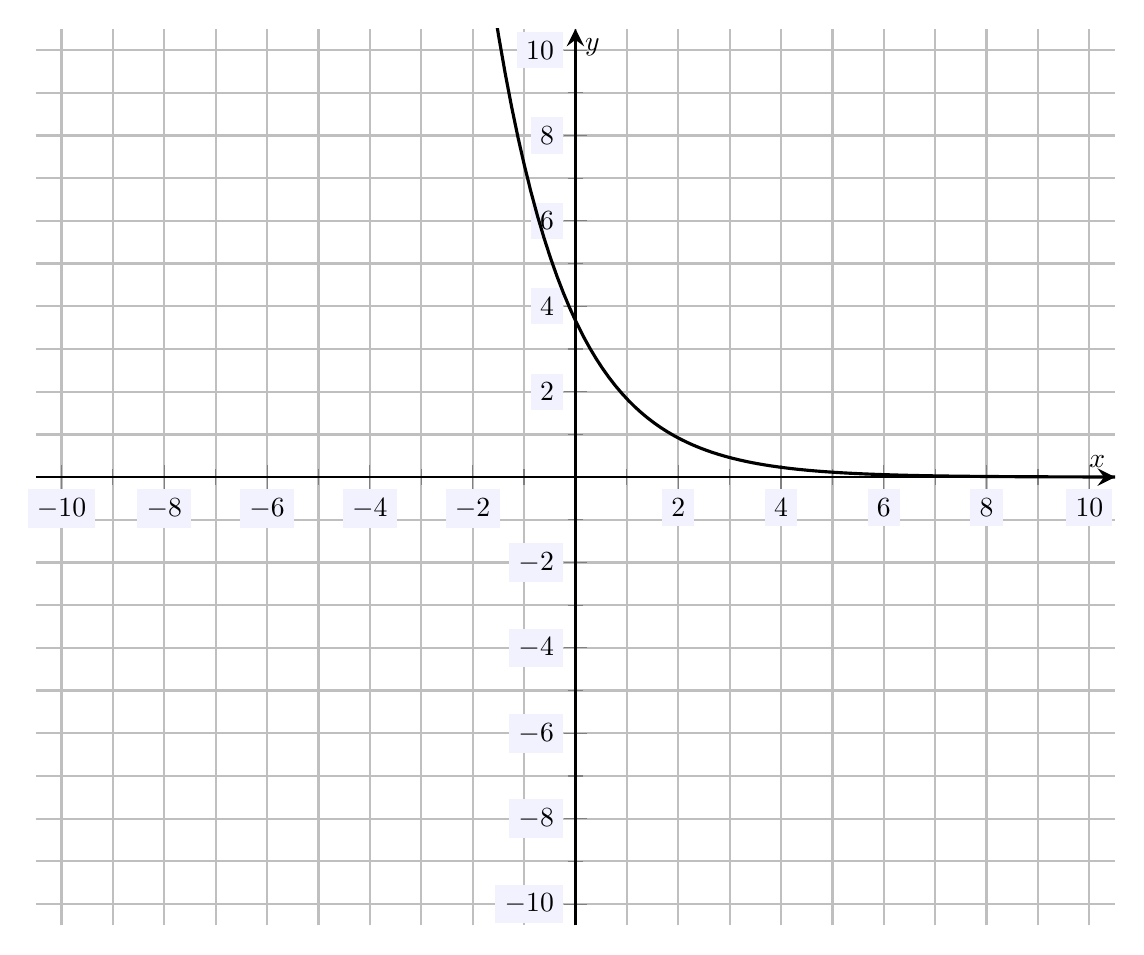
\begin{tikzpicture}[scale=2,every node/.style={scale=0.5}]
	\begin{axis}[
	grid=both,
	axis lines=middle,
	ticklabel style={fill=blue!5!white},
	xmin= -10.5, xmax=10.5,
	ymin= -10.5, ymax=10.5,
	xtick={-10,-8,-6,-4,-2,0,2,4,6,8,10},
	ytick={-10,-8,-6,-4,-2,0,2,4,6,8,10},
	minor tick = {-10,-9,...,10},
	xlabel=\(x\),ylabel=\(y\),
	]
	\addplot[line width= 0.02cm,domain= -2:10.5,samples=100] ({x},{11/3*(1/2)^x}); 
	\end{axis}
	\end{tikzpicture}
	}
	\] \pspace

\sol The function $f(x)= \dfrac{11}{3} \left( \dfrac{1}{2} \right)^x$ is in the form $Ab^{cx}$. Because $b= \frac{1}{2} < 1$, $c= 1 > 0$, and $a= \frac{11}{3} > 0$, we know that the function $f(x)$ is decreasing. Because $a > 0$, we know that $f(x)$ is always positive. We know also that the $y$-intercept is given by $f(0)= \frac{11}{3} \left( \frac{1}{2} \right)^0= \frac{11}{3} \cdot 1= \frac{11}{3}$, so that the $y$-intercept is $(0, \frac{11}{3})$. Putting this information gives the sketch above. 



\newpage



% Problem 2
\problem{10} Showing all your work, determine whether the following functions are increasing or decreasing:
	\begin{enumerate}[(a)]
	\item $-5 \left( 2 \right)^{-\frac{1}{5} x}$
	\item $\dfrac{7}{8} \left( \dfrac{5}{6} \right)^{4x}$
	\item $17 \left( \dfrac{5}{4} \right)^{-x}$
	\item $-10 \left( \dfrac{1}{3} \right)^{-5x}$
	\end{enumerate} \pspace

\sol
\begin{enumerate}[(a)]
\item The function $-5 \left( 2 \right)^{-\frac{1}{5} x}$ is in the form $Ab^{cx}$. Because $b= 2 > 1$, $c= -\frac{1}{5} < 0$, and $a= -5 < 0$, we know that the function is increasing. 

\item The function $\dfrac{7}{8} \left( \dfrac{5}{6} \right)^{4x}$ is in the form $Ab^{cx}$. Because $b= \frac{5}{6} < 1$, $c= 4 > 0$, and $a= \frac{7}{8} > 0$, we know that the function is decreasing. 

\item The function $17 \left( \dfrac{5}{4} \right)^{-x}$ is in the form $Ab^{cx}$. Because $b= \frac{5}{4} > 1$, $c= -1 < 0$, and $a= 17 > 0$, we know that the function is decreasing. 

\item The function $-10 \left( \dfrac{1}{3} \right)^{-5x}$ is in the form $Ab^{cx}$. Because $b= \frac{1}{3} < 1$, $c= -5 < 0$, and $a= -10 < 0$, we know that the function is decreasing. 
\end{enumerate}



\newpage



% Problem 3
\problem{10} Showing all your work, solve the following equation:
	\[
	2^{3x}= 4
	\] \pspace

\sol
	\begin{gather*}
	2^{3x}= 4 \\[0.3cm]
	2^{3x}= 2^2 \\[0.3cm]
	3x= 2 \\[0.3cm]
	x= \dfrac{2}{3}
	\end{gather*}



\newpage



% Problem 4
\problem{10} Showing all your work, solve the following equation:
	\[
	7(4^{1 - x})= \dfrac{7}{16}
	\] \pspace

\sol
	\begin{gather*}
	7(4^{1 - x})= \dfrac{7}{16} \\[0.3cm]
	\dfrac{1}{7} \cdot 7(4^{1 - x})= \dfrac{7}{16} \cdot \dfrac{1}{7} \\[0.3cm]
	4^{1 - x}= \dfrac{1}{16} \\[0.3cm]
	2^{2(1 - x)}= 2^{-4} \\[0.3cm]
	2(1 - x)= -4 \\[0.3cm]
	1 - x= -2 \\[0.3cm]
	x= 3
	\end{gather*}



\newpage



% Problem 5
\problem{10} Showing all your work, solve the following equation:
	\[
	\dfrac{1}{3^x}= 27^{\frac{4x + 10}{3}}
	\] \pspace

\sol
	\begin{gather*}
	\dfrac{1}{3^x}= 27^{\frac{4x + 10}{3}} \\[0.3cm]
	3^{-x}= 3^{3 \cdot \frac{4x + 10}{3}} \\[0.3cm]
	-x= 4x + 10 \\[0.3cm]
	-5x= 10 \\[0.3cm]
	x= -2
	\end{gather*}



\newpage



% Problem 6
\problem{10} Showing all your work, solve the following equation:
	\[
	5^{x - 2} + 6= 11
	\] \pspace

\sol
	\begin{gather*}
	5^{x - 2} + 6= 11 \\[0.3cm]
	5^{x - 2}= 5^1 \\[0.3cm]
	x - 2= 1 \\[0.3cm]
	x= 3
	\end{gather*}



\newpage



% Problem 7
\problem{10} Showing all your work, solve the following equation:
	\[
	\dfrac{1}{4^x}= 1024
	\] \pspace

\sol
	\begin{gather*}
	\dfrac{1}{4^x}= 1024 \\[0.3cm]
	4^{-x}= 4^{5} \\[0.3cm]
	-x= 5 \\[0.3cm]
	x= -5
	\end{gather*}



\newpage



% Problem 8
\problem{10} Showing all your work, solve the following equation:
	\[
	\left( \dfrac{2}{3} \right)^{5x - 7}= 1
	\] \pspace

\sol
	\begin{gather*}
	\left( \dfrac{2}{3} \right)^{5x - 7}= 1 \\[0.3cm]
	\left( \dfrac{2}{3} \right)^{5x - 7}= \left( \dfrac{2}{3} \right)^0 \\[0.3cm]
	5x - 7= 0 \\[0.3cm]
	5x= 7 \\[0.3cm]
	x= \dfrac{7}{5}
	\end{gather*}



\newpage



% Problem 9
\problem{10} Suppose you invest \$5,000 in an account which earns 4.6\% annual interest, compounded quarterly. How much will be in the account after 3~years? \pspace

\sol If $P$ dollars are placed in an account which earns yearly interest at a rate $r$, compounded $k$ times per year, then the amount of money in the account after $t$ years, $F$, is given by \pspace
	\[
	F= P \left(1 + \dfrac{r}{k} \right)^{kt}
	\] \pspace
Here, we have $P= 5000$, $r= 0.046$, $k= 4$, and $t= 3$. But then we have\dots \pspace
	\[
	F= P \left(1 + \dfrac{r}{k} \right)^{kt}= 5000 \left( 1 + \dfrac{0.046}{4} \right)^{4 \cdot 3}= 5000 (1.0115)^{12}= 5000(1.14707191)= 5735.36
	\] \pspace
Therefore, the account will have \$5,735.36. 



\newpage


% Problem 10
\problem{10} If you take out a loan for \$1,200 at a 5.5\% annual interest, compounded continuously, how much is owed after 2~years? How much of this amount is interest? \pspace

\sol If $P$ dollars are taken out on a loan with interest rate $r$, then the amount of money owed on the loan after $t$ years, $F$, is given by \pspace
	\[
	F= P e^{rt}
	\] \pspace
Here, we have $P= 1200$, $r= 0.055$, and $t= 2$. Then\dots \pspace
	\[
	F= Pe^{rt}= 1200 e^{0.055 \cdot 2}= 1200 e^{0.11}= 1200(1.11627807)= 1339.53
	\] \pspace
Therefore, you will owe \$1,339.53 on the loan after 2~years. 


\end{document}